\documentclass[border=4pt]{standalone}
\usepackage[T1]{fontenc}
\usepackage{tikz}
\usetikzlibrary{arrows.meta,positioning,fit,backgrounds,shapes.geometric,calc}
\definecolor{orch}{HTML}{234767}
\definecolor{ctx}{HTML}{EAF1F8}
\definecolor{retr}{HTML}{E2F0ED}
\definecolor{ext}{HTML}{F7EBDD}
\definecolor{infra}{HTML}{F1F3F5}
\tikzset{
 every node/.style={font=\sffamily\fontsize{8.5}{10}\selectfont,align=center,execute at begin node={\hyphenpenalty=10000\exhyphenpenalty=10000}},
 block/.style={draw=orch!80,fill=white,rounded corners=1.5pt,minimum height=7mm,inner sep=3pt,line width=.55pt},
 context/.style={block,fill=ctx},
 engine/.style={block,fill=orch,text=white},
 retrieval/.style={block,fill=retr},
 external/.style={block,fill=ext},
 storage/.style={block,fill=infra},
 optional/.style={dashed},
 flow/.style={-{Stealth[length=2mm]},draw=orch!90,line width=.65pt},
 control/.style={flow,dashed},
 error/.style={flow,densely dotted},
 group/.style={draw=orch!50,rounded corners=3pt,inner sep=5pt,line width=.5pt},
 heading/.style={font=\sffamily\bfseries\fontsize{8.5}{10}\selectfont,text=orch},
 edgelabel/.style={font=\sffamily\fontsize{7.5}{9}\selectfont,fill=white,inner sep=1pt,text=orch}
}

\begin{document}
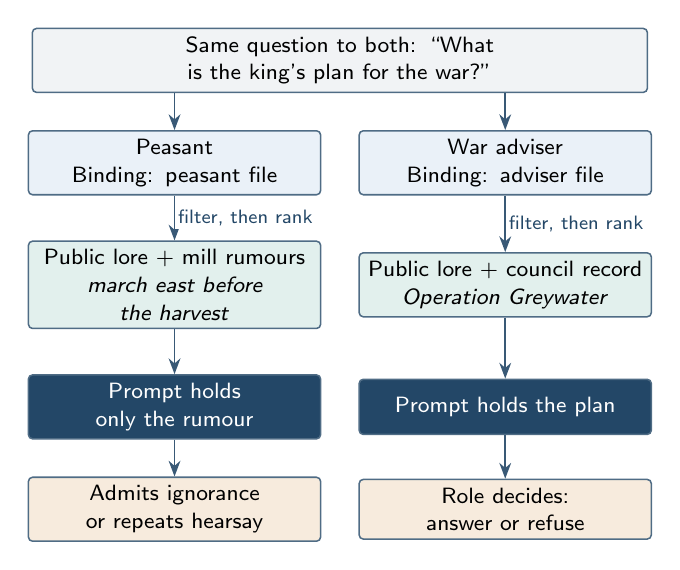
\begin{tikzpicture}
\node[storage,text width=7.6cm] (q) at (0,4.9) {Same question to both: ``What is the king's plan for the war?''};
\node[context,text width=3.5cm] (p) at (-2.1,3.6) {Peasant\\Binding: peasant file};
\node[context,text width=3.5cm] (a) at (2.1,3.6) {War adviser\\Binding: adviser file};
\node[retrieval,text width=3.5cm] (pd) at (-2.1,2.05) {Public lore + mill rumours\\\textit{march east before the harvest}};
\node[retrieval,text width=3.5cm] (ad) at (2.1,2.05) {Public lore + council record\\\textit{Operation Greywater}};
\node[engine,text width=3.5cm] (pr) at (-2.1,.5) {Prompt holds only the rumour};
\node[engine,text width=3.5cm] (ar) at (2.1,.5) {Prompt holds the plan};
\node[external,text width=3.5cm] (po) at (-2.1,-.8) {Admits ignorance or repeats hearsay};
\node[external,text width=3.5cm] (ao) at (2.1,-.8) {Role decides: answer or refuse};
\draw[flow] (q.south -| p) -- (p);
\draw[flow] (q.south -| a) -- (a);
\draw[flow] (p) -- node[edgelabel,right]{filter, then rank} (pd);
\draw[flow] (a) -- node[edgelabel,right]{filter, then rank} (ad);
\draw[flow] (pd) -- (pr);
\draw[flow] (ad) -- (ar);
\draw[flow] (pr) -- (po);
\draw[flow] (ar) -- (ao);
\end{tikzpicture}
\end{document}
